% English draft based on sections/03_nonclosure_theorem_ja.tex
\section{The Non-Closure Theorem: No Internal Fixed Point in $L_F$}

\noindent\textbf{Scope of the account.} The theorem discussion is conditional on the stated strict increase of justification and the fixed-constraint, within-region scope. No proof-validity certification or universal cognitive interpretation is supplied here. The hypothetical binary stopping predicate models stopping as a fixed-point condition; its applicability to arbitrary cognitive cessation and the reapplication of the premises to auxiliary inference remain open. Boundary divergence and fixed-point absence are compared by role, not as a proved isomorphism. Individual closure failure, external stopping necessity, and collapse regimes are separate architectural or cognitive hypotheses.


This chapter is the first center of the paper. It preserves the historical local-state model's conditional fixed-point claim for the inference layer $L_F$. Externalized stopping is a separate architecture proposal, not a universal consequence of that claim.

\noindent\textbf{Historical local-model boundary.} In this chapter, references to inference F, scalar justification J, and their fixed-point consequences belong to the preserved local-state model, not to the active record/position contract of Section 2. The following C-landscape figure depicts that old scalar-J, fixed-constraint conditional argument, not a proof of the new position interface. The original premises, theorem, proof, and later corollaries are retained as historical material: only the old admissible-domain kernel is at issue; broader readings remain on hold. No proof transfers to the new contract, and fresh occurrence identifiers supply no substantive no-fixed-point theorem. This attribution extends to the old-model references throughout this chapter, not to a retyping of the closure PDE or field-flow vocabulary.

\begin{figure}[H]
\centering
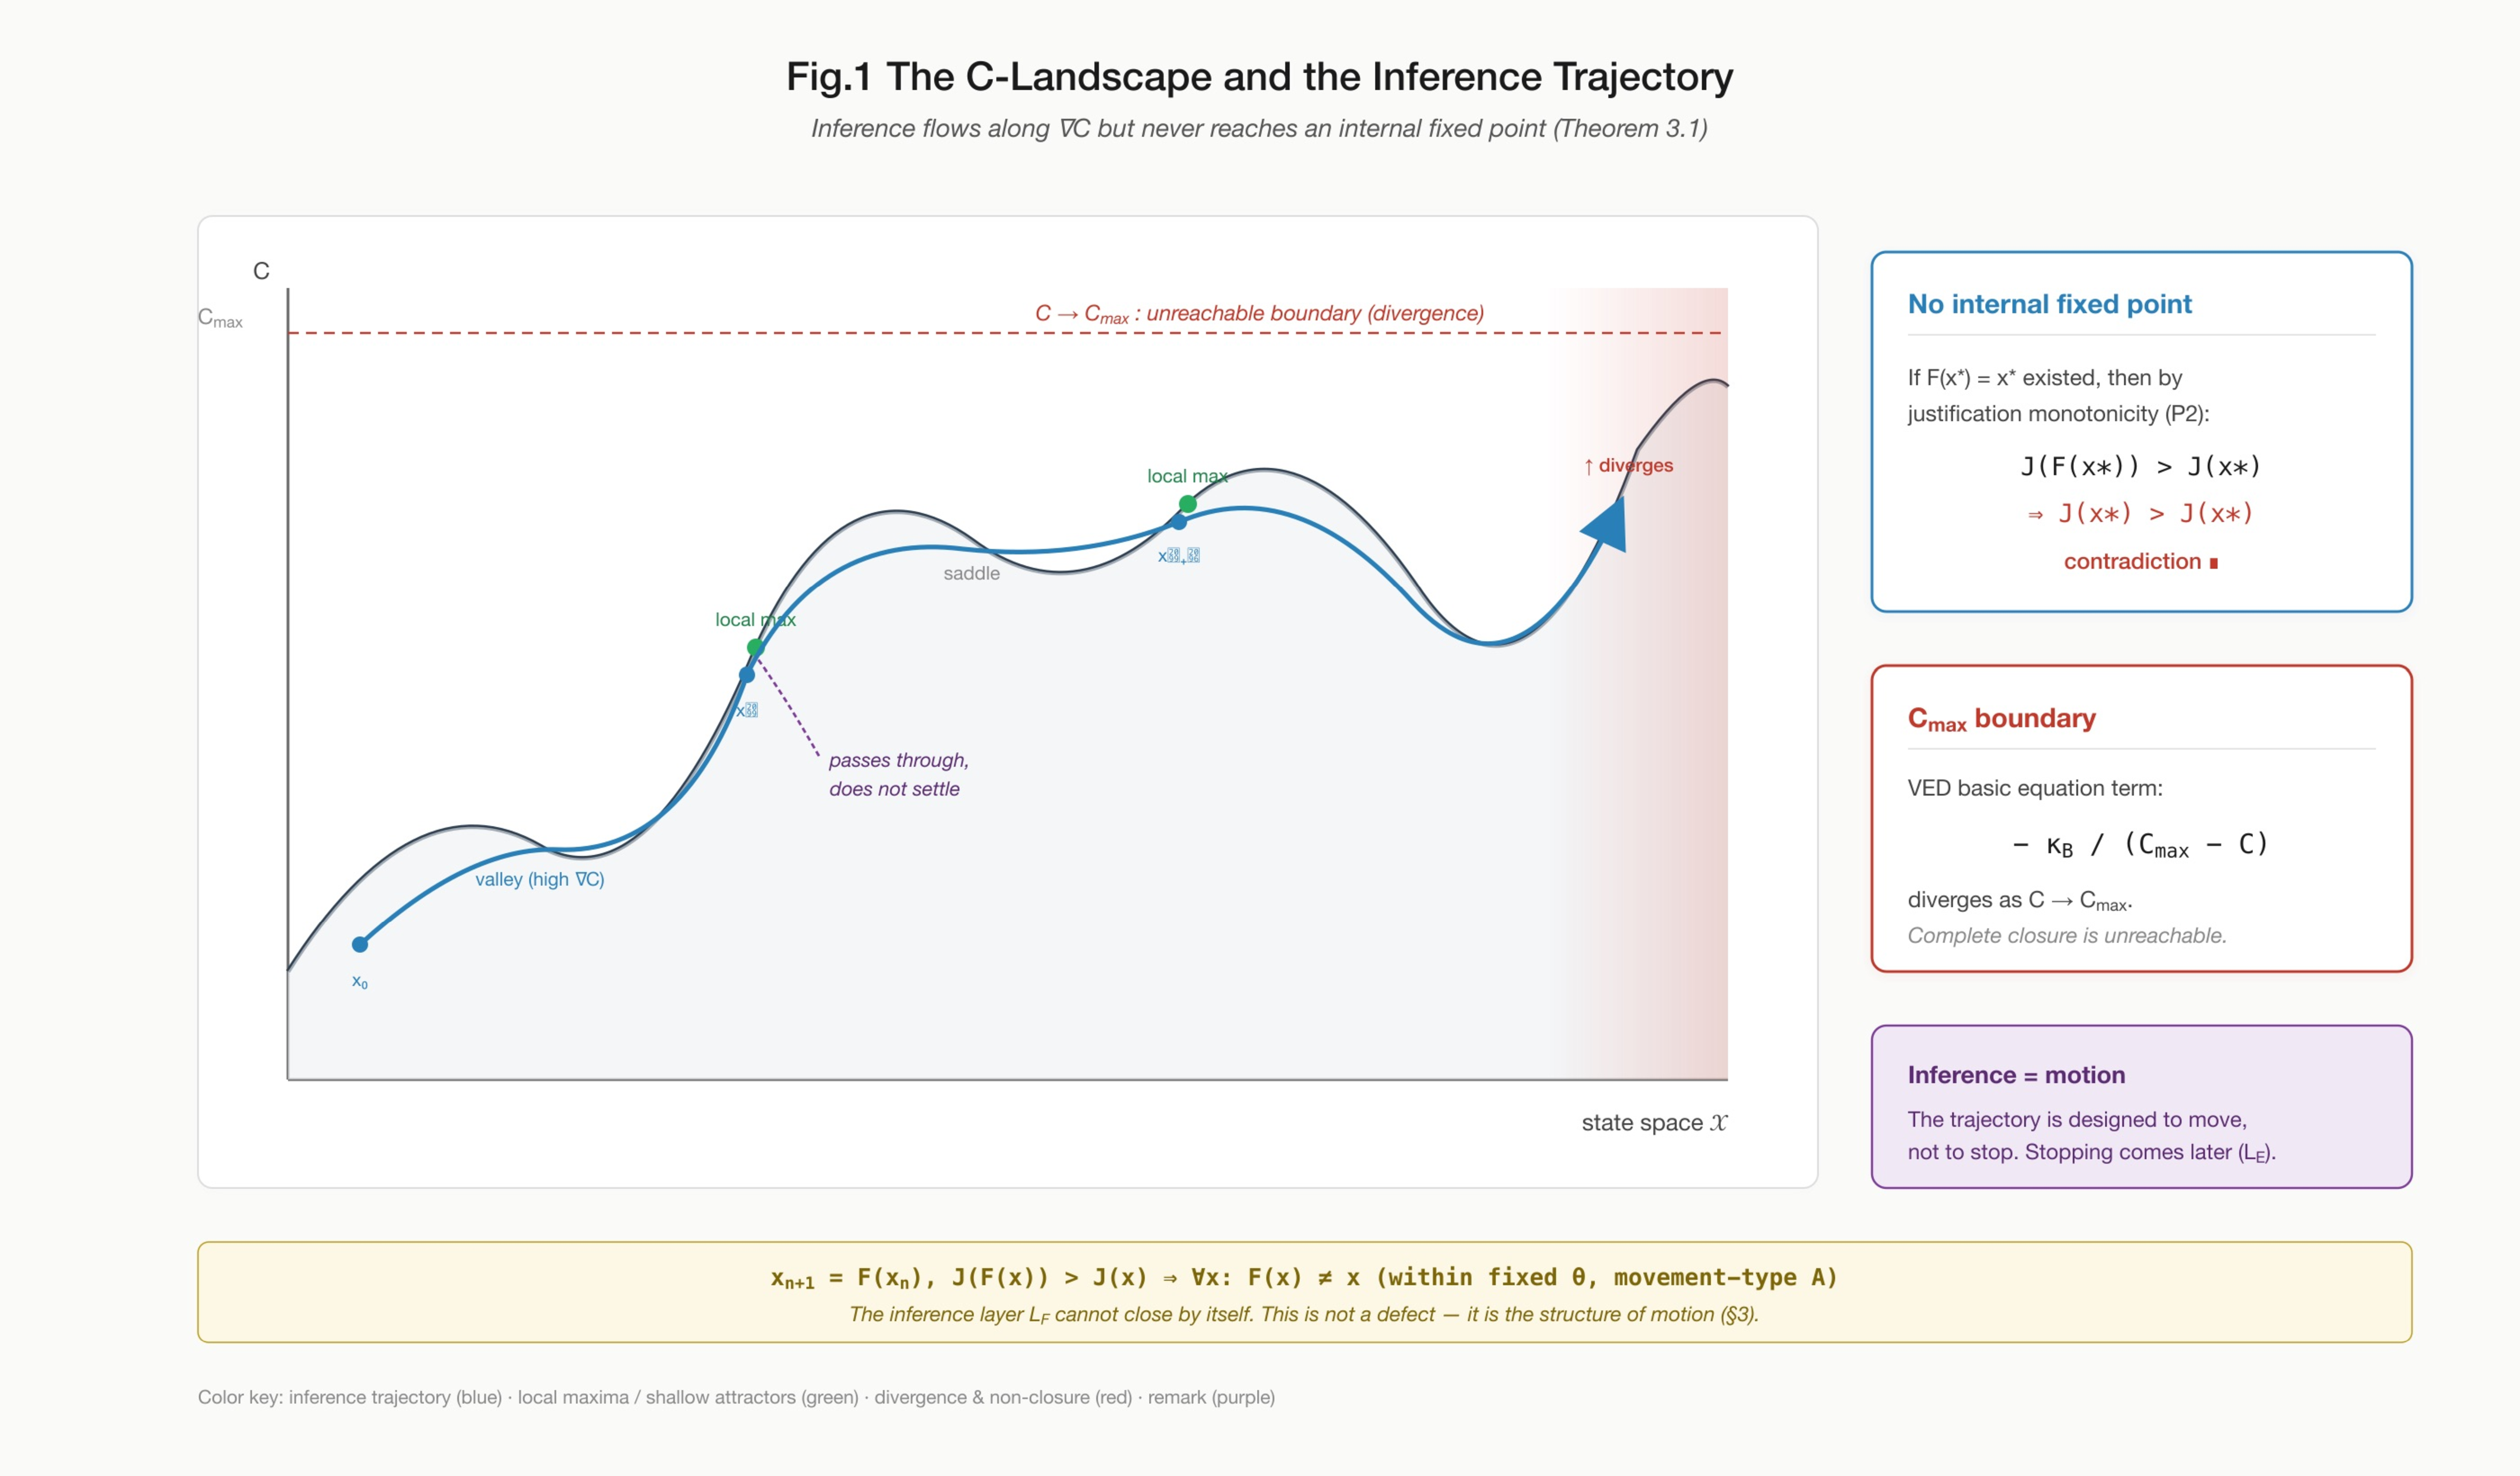
\includegraphics[width=\linewidth]{fig1_c_landscape.pdf}
\caption{Schematic C-landscape and inference trajectory along $\nabla C$. The conditional fixed-point discussion does not establish the impossibility of every cognitive stopping event.}
\label{fig:part2-c-landscape}
\figurenote{The horizontal axis is state space and the vertical axis is closure degree $C$. The blue trajectory represents iterations of $F$, while the red boundary marks the proposed boundary $C_{\max}$; dynamic inaccessibility is not established.}{Under the stated strict-justification premise, within fixed $\theta$ and movement type (A), $L_F$ has no internal fixed point. The figure motivates comparison with $\mu_\theta$, region reconfiguration, and $L_E$, not their necessity or existence.}
\end{figure}

\subsection{Assumptions}

The following sketch uses the stated assumptions; their general cognitive applicability is not established.

\textbf{P1: Justification extension.} The inference operator $F$ sends a state $x_n$ to a more justified state $x_{n+1}=F(x_n)$.

\textbf{P2: Monotonic justification measure.} There exists a measure $J$ such that
\[
J(F(x))>J(x)
\]
for admissible states.

\textbf{P3: Fixed movement region.} The argument is made within a fixed movement region $\Omega_\theta$. It concerns movement type (A), not reconfiguration type (B).

\subsection{Theorem}

\textbf{Theorem 3.1 (Non-Closure Theorem).}
For any inference operator $F$ satisfying P1 and P2, there is no internal fixed point $x^*$ such that
\[
F(x^*)=x^*.
\]
Equivalently,
\[
\forall x\in\mathcal{X},\quad F(x)\neq x
\]
within the range of fixed-$\theta$ inference.

\subsection{Proof Sketch}

Assume, for contradiction, that a fixed point $x^*$ exists. Then $F(x^*)=x^*$. By P2,
\[
J(F(x^*))>J(x^*).
\]
But since $F(x^*)=x^*$, this becomes
\[
J(x^*)>J(x^*),
\]
which is impossible. Therefore no such internal fixed point exists.

The proof is short because the result follows from the minimal meaning of inference as justification extension. The exclusion concerns the specified fixed-point model. It does not exclude every independently defined cognitive stop.

\subsection{Branching Explosion}

Fixed-point absence and branching are distinct claims. The former concerns the historical conditional local-state model; the latter is a proposed interpretation of some probabilistic or generative inference processes, not a consequence of fixed-point absence alone.

Within that historical account, this is compared by role with the branching explosion introduced in Part I. Interpreting it as a failure of cognitive stopping requires a separate bridge that is not established here. The increase of inferential capacity may therefore accelerate branching explosion rather than suppress it. The problem of intelligence shifts from strengthening inference itself to operating enlarged branching in a stoppable form.

\subsection{Consequence}

In that historical model, the inference layer $L_F$ is not the whole of the proposed architecture. Regress or explosion is a cognitive hypothesis, not a general consequence established by the fixed-point result. Requiring further inference for an internal predicate is part of the stopping model under discussion; its applicability to arbitrary cognitive stopping remains open. Stopping outside $F$ is proposed as an architectural option. \S{}5 develops a hypothesis involving $L_R$ and $L_E$, without establishing their generation.

\bigskip
